\documentclass{article}
\usepackage{fullpage}
\usepackage{listings}
\usepackage{color}
\usepackage{graphicx}
\usepackage[ngerman]{babel}
\usepackage[utf8]{inputenc}
\usepackage{float}
\usepackage{hyperref}

\definecolor{mygreen}{rgb}{0,0.6,0}
\definecolor{mygray}{rgb}{0.5,0.5,0.5}
\definecolor{mymauve}{rgb}{0.58,0,0.82}

\lstset{
  backgroundcolor=\color{white},
  basicstyle=\footnotesize,
  breakatwhitespace=false,
  breaklines=true,
  captionpos=b,
  commentstyle=\color{mygreen},
  deletekeywords={...},
  escapeinside={\%*}{*)},
  extendedchars=true,
  frame=single,
  keepspaces=true,
  keywordstyle=\color{blue},
  language=C,
  morekeywords={*,...},
  numbers=left,
  numbersep=5pt,
  numberstyle=\tiny\color{mygray},
  rulecolor=\color{black},
  showspaces=false,
  showstringspaces=false,
  showtabs=false,
  stepnumber=2,
  stringstyle=\color{mymauve},
  tabsize=2,
  title=\lstname
}
\usepackage{CJKutf8}
\usepackage{pdfpages}

\begin{document}

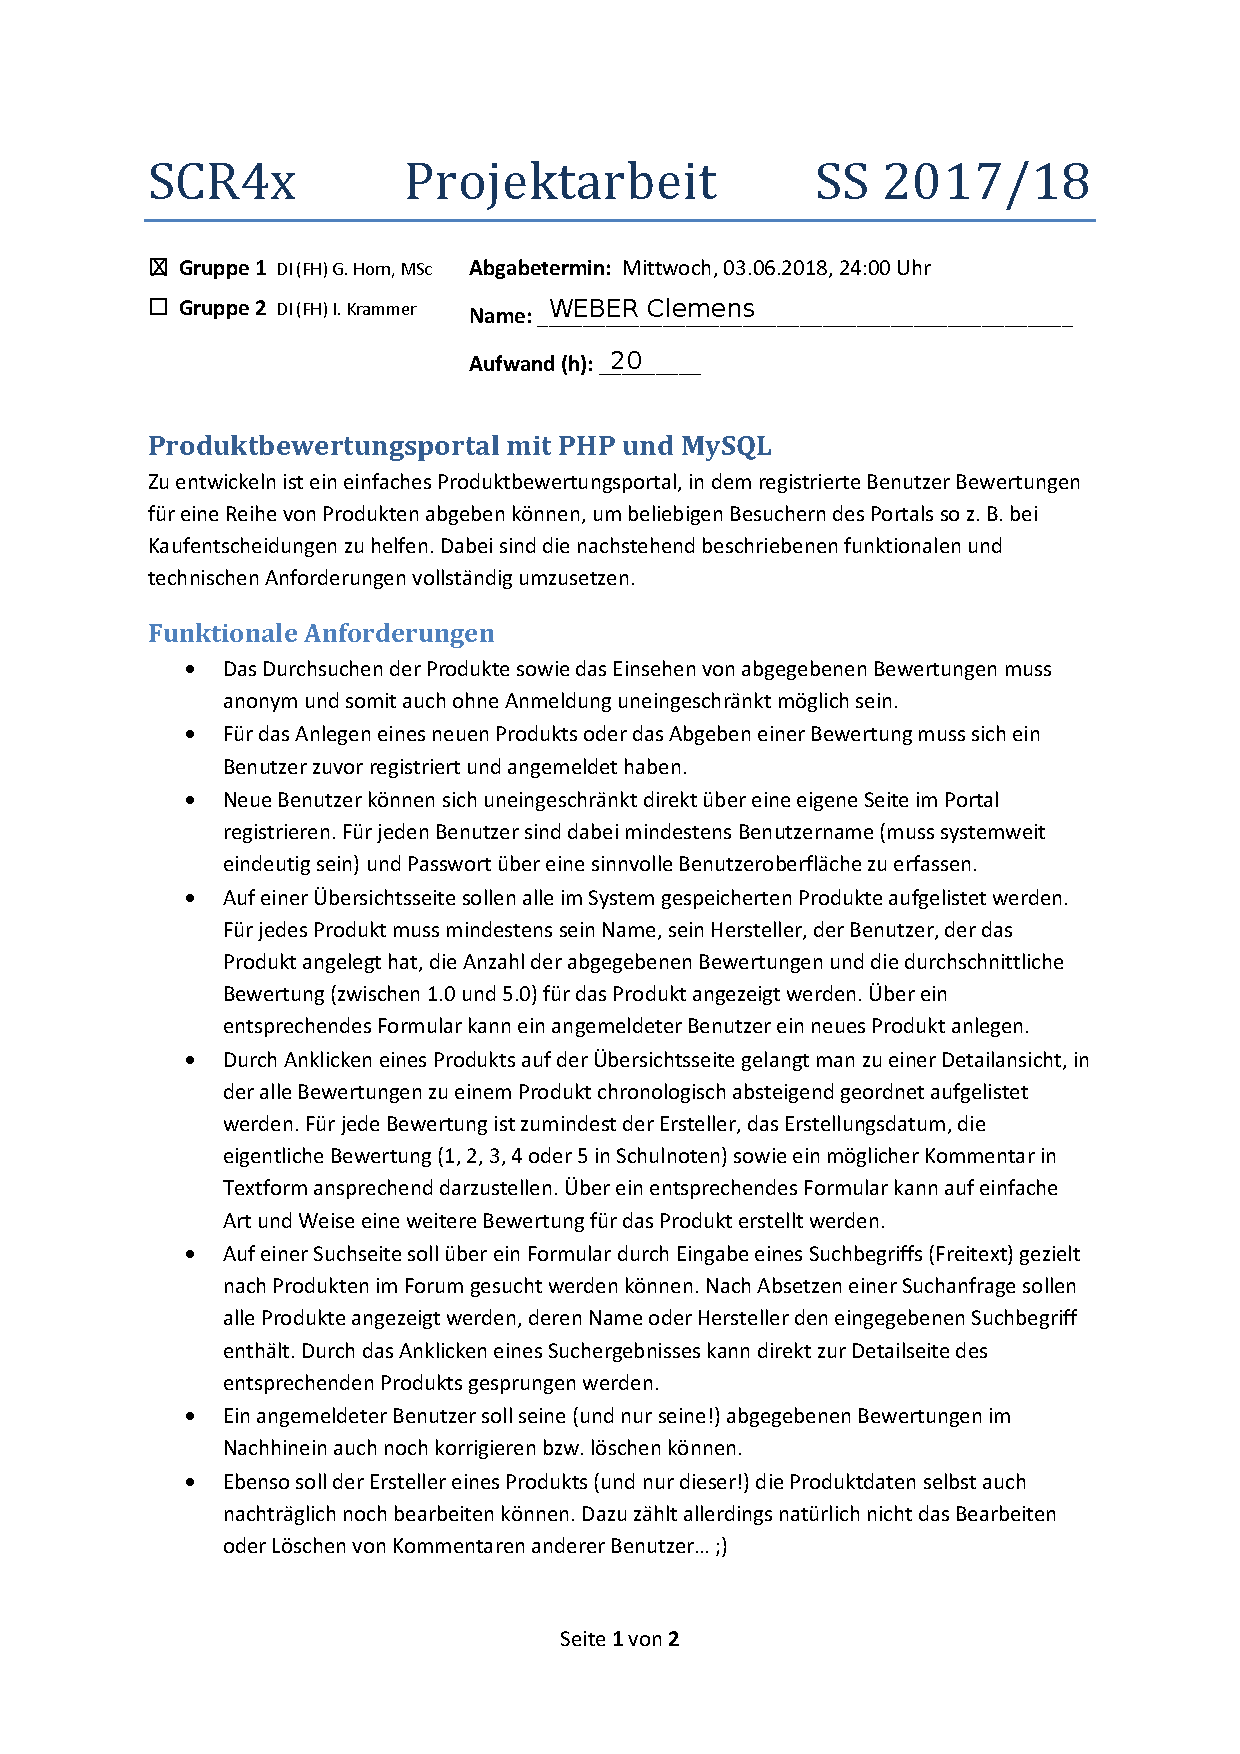
\includepdf[pages=-]{angabe.pdf}

\section{Produktwebertungportal}

\subsection{Lösungsidee}
Wie in der Angabe vorgegeben wurde das MVC Muster angewandt. Sowohl
die Struktur als auch zum Teil der Code wurden von der Übung übernommen.
Das Model besteht aus den Entitäten User, Product und Rating. Die
Repräsentation in der Datenbank kann im Bild weiter unten entnommen werden.
Auf der Hauptseite befindet sich eine Liste mit allen Produkten sowie
die Möglichkeit die angezeigten Produkte zu filtern. Wird auf ein Produkt
geklickt, so wird die Detailansicht geöffnet. Erst wenn sich ein Benutzer
registriert und angemeldet hat, erscheint die Schaltfläche um ein neues
Produkt anzulegen. In der Detailansicht wird nach der Anmeldung ebenfalls
eine Schaltfläche aktiviert um ein Rating abzugeben.

\subsection{Datenbank}

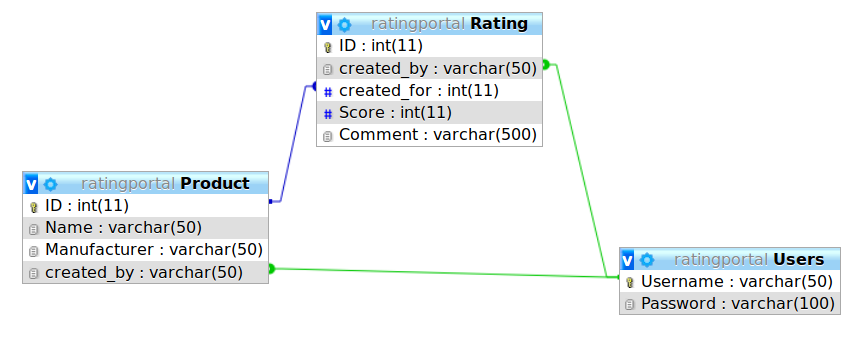
\includegraphics[width=1.0\textwidth]{dbmodel.png}

\lstinputlisting{../database/create.txt}
\lstinputlisting{../database/testdata.txt}

\subsection{Sourcecode}

\lstinputlisting[language=PHP]{../index.php}
\lstinputlisting[language=PHP]{../src/BusinessLogic/AuthenticationManager.php}
\lstinputlisting[language=PHP]{../src/BusinessLogic/Session.php}
\lstinputlisting[language=PHP]{../src/Controllers/Home.php}
\lstinputlisting[language=PHP]{../src/Controllers/NewProduct.php}
\lstinputlisting[language=PHP]{../src/Controllers/NewRating.php}
\lstinputlisting[language=PHP]{../src/Controllers/Product.php}
\lstinputlisting[language=PHP]{../src/Controllers/User.php}
\lstinputlisting[language=PHP]{../src/Controllers/UserHome.php}
\lstinputlisting[language=PHP]{../src/DataLayer/DataLayer.php}
\lstinputlisting[language=PHP]{../src/DataLayer/DBDataLayer.php}
\lstinputlisting[language=PHP]{../src/Domain/Entity.php}
\lstinputlisting[language=PHP]{../src/Domain/Product.php}
\lstinputlisting[language=PHP]{../src/Domain/Rating.php}
\lstinputlisting[language=PHP]{../src/Domain/User.php}
\lstinputlisting[language=PHP]{../src/Framework/Controller.php}
\lstinputlisting[language=PHP]{../src/Framework/Injector.php}
\lstinputlisting[language=PHP]{../src/Framework/MVC.php}
\lstinputlisting[language=PHP]{../src/Framework/ViewRenderer.php}
\lstinputlisting[language=PHP]{../views/home.inc}
\lstinputlisting[language=PHP]{../views/login.inc}
\lstinputlisting[language=PHP]{../views/newproduct.inc}
\lstinputlisting[language=PHP]{../views/newrating.inc}
\lstinputlisting[language=PHP]{../views/product.inc}
\lstinputlisting[language=PHP]{../views/register.inc}
\lstinputlisting[language=PHP]{../views/userhome.inc}
\lstinputlisting[language=PHP]{../views/partial/errors.inc}
\lstinputlisting[language=PHP]{../views/partial/footer.inc}
\lstinputlisting[language=PHP]{../views/partial/header.inc}
\lstinputlisting[language=PHP]{../views/partial/user.inc}

\subsection{Tests}


Übersichtsseite der Produkte, nicht eingeloggt.

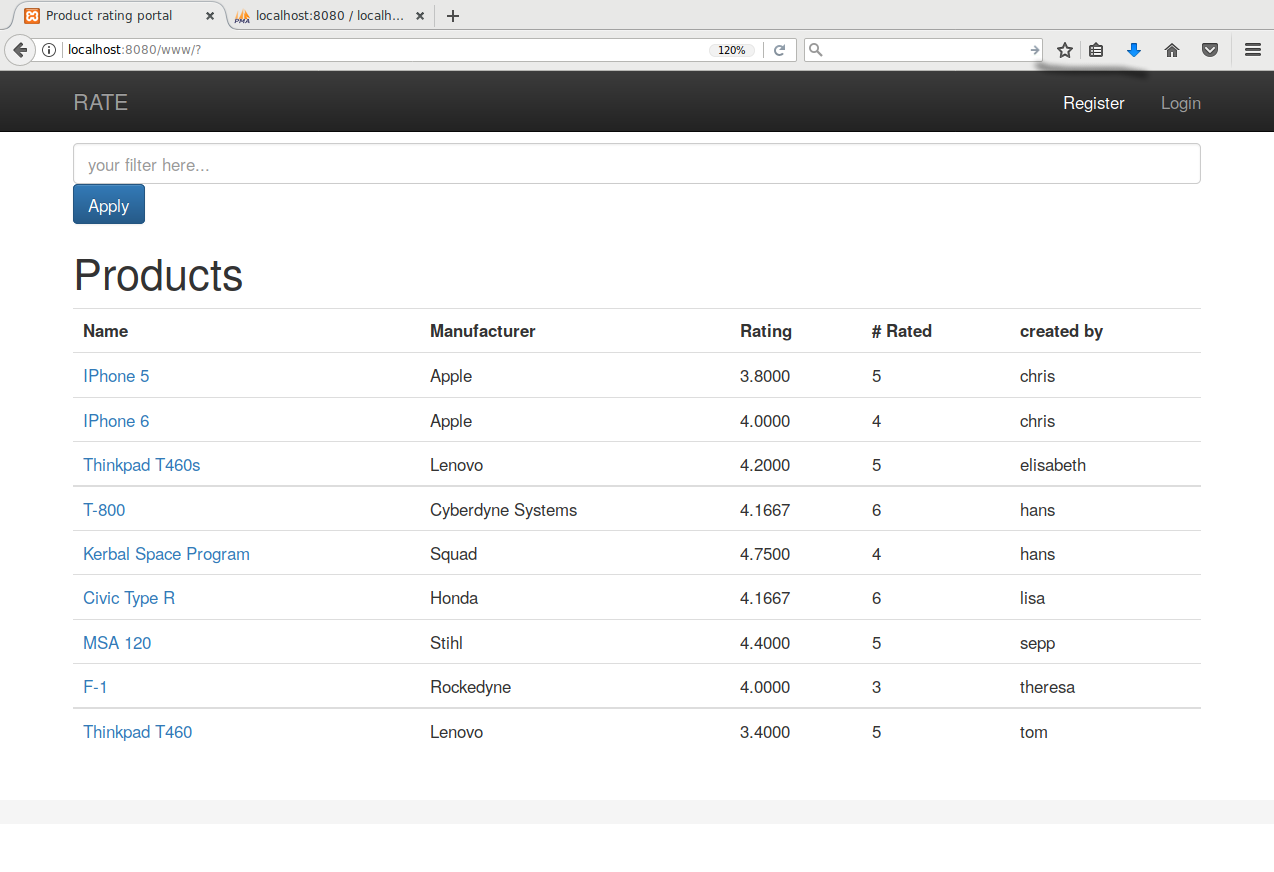
\includegraphics[width=1.0\textwidth]{1.png}

Registrierungsmaske; Fehler bei ungültiger Eingabe.

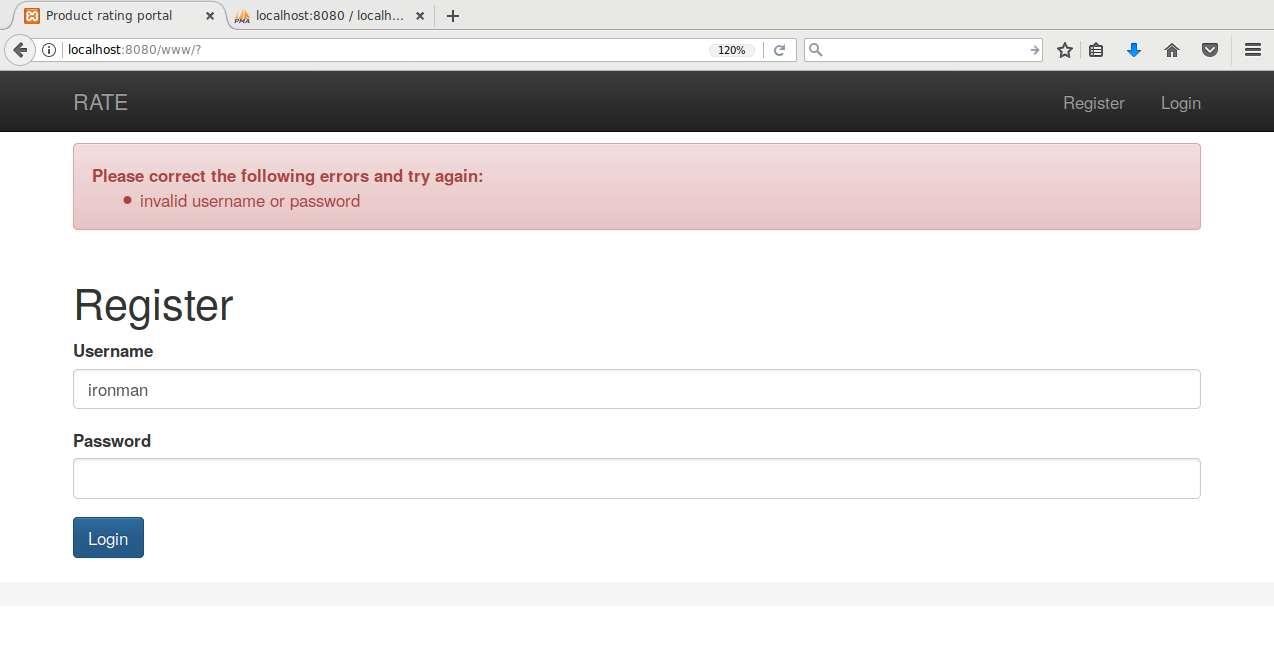
\includegraphics[width=1.0\textwidth]{2.png}

Nach erfolgreicher registrierung Weiterleitung auf Login-Maske.

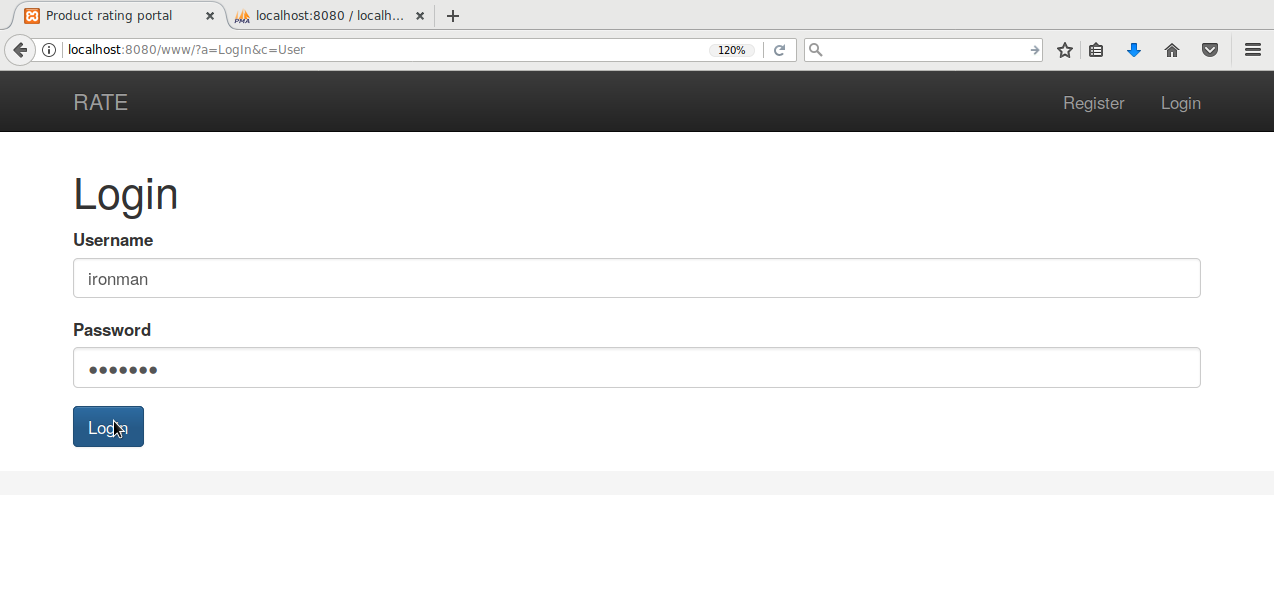
\includegraphics[width=1.0\textwidth]{3.png}

Übersichtsseite nach erfolgreichem Login.

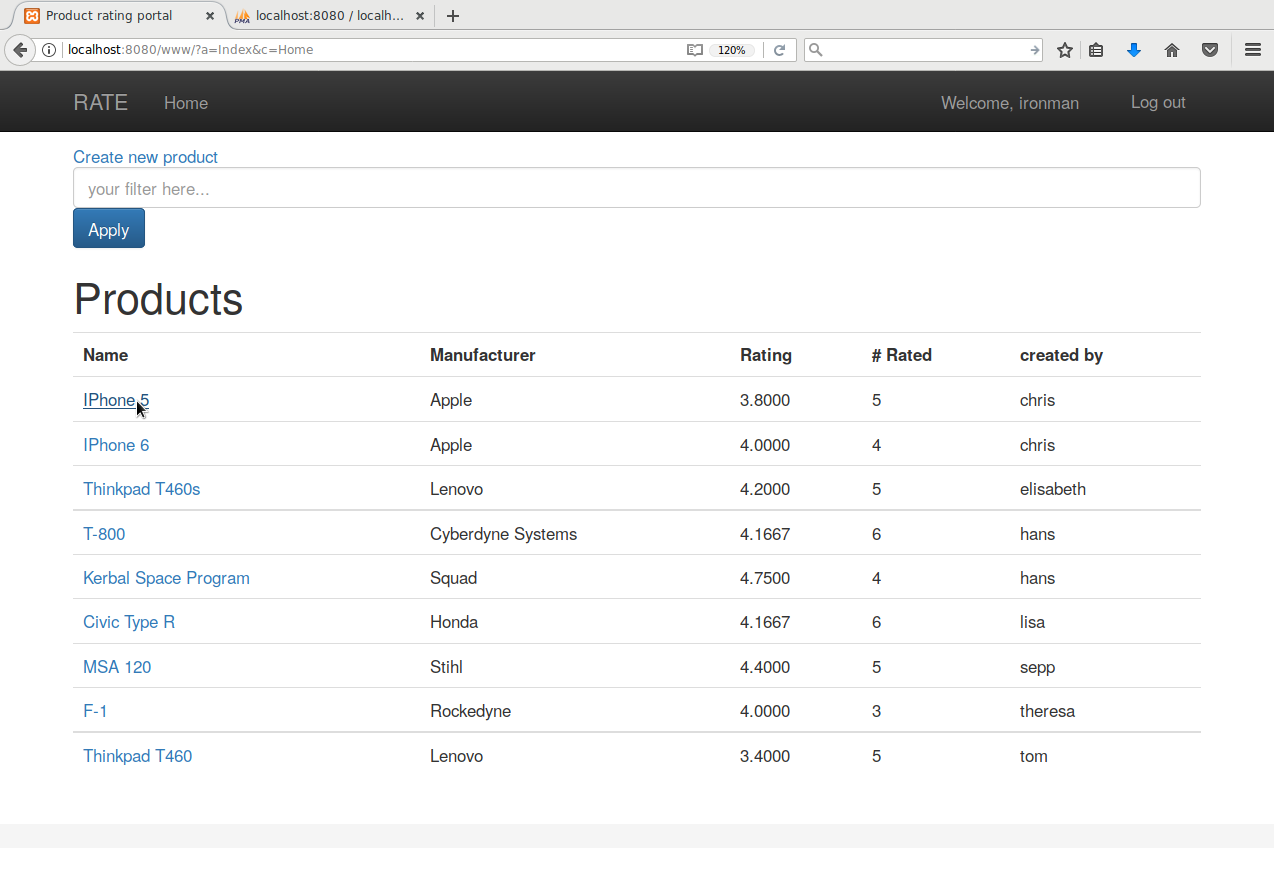
\includegraphics[width=1.0\textwidth]{4.png}

Detailansicht eines Produkts.

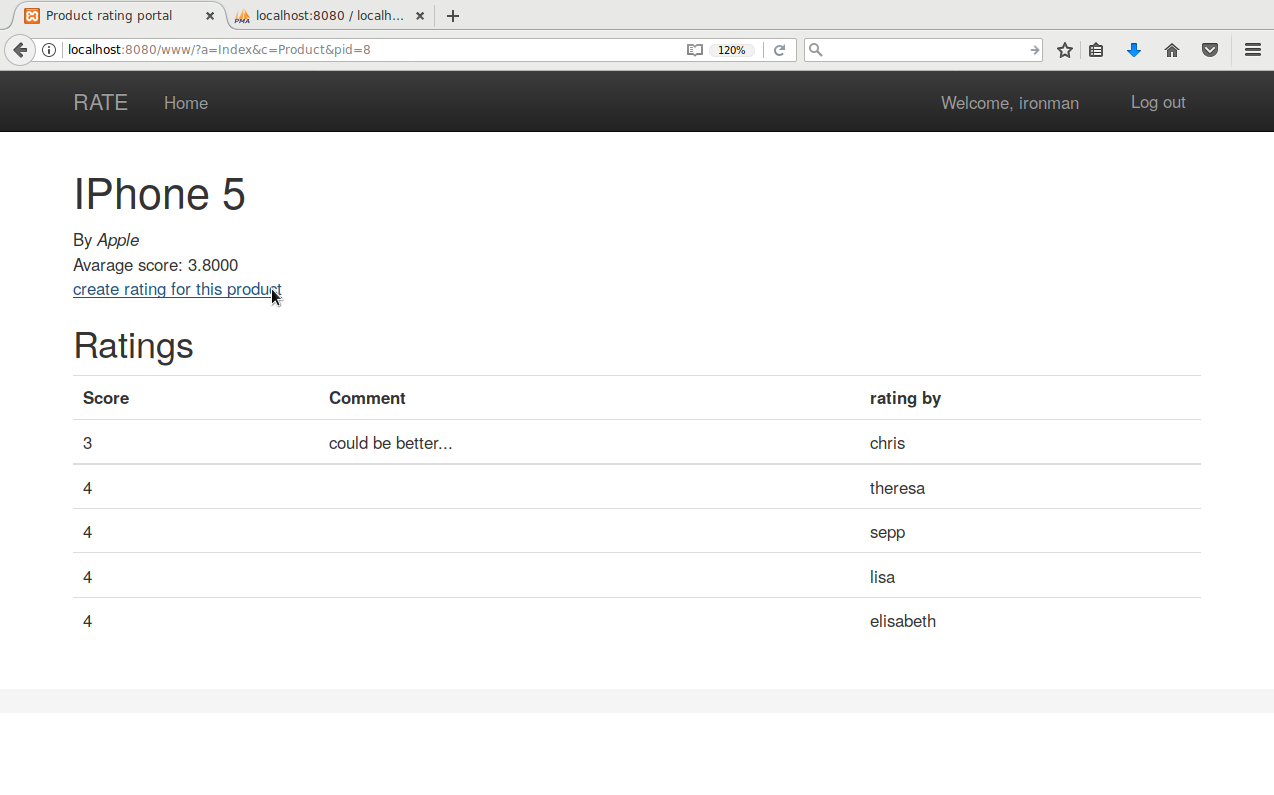
\includegraphics[width=1.0\textwidth]{5.png}

Erstellung einer neuen Bewertung.

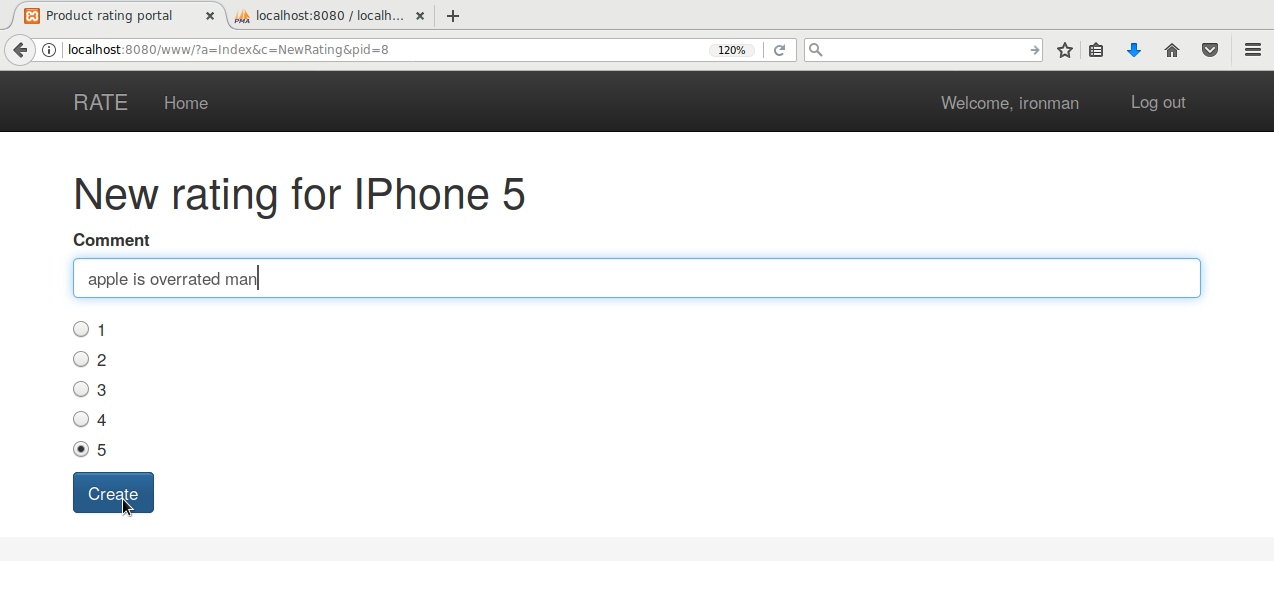
\includegraphics[width=1.0\textwidth]{6.png}

Detailansicht mit neuer Bewertung.

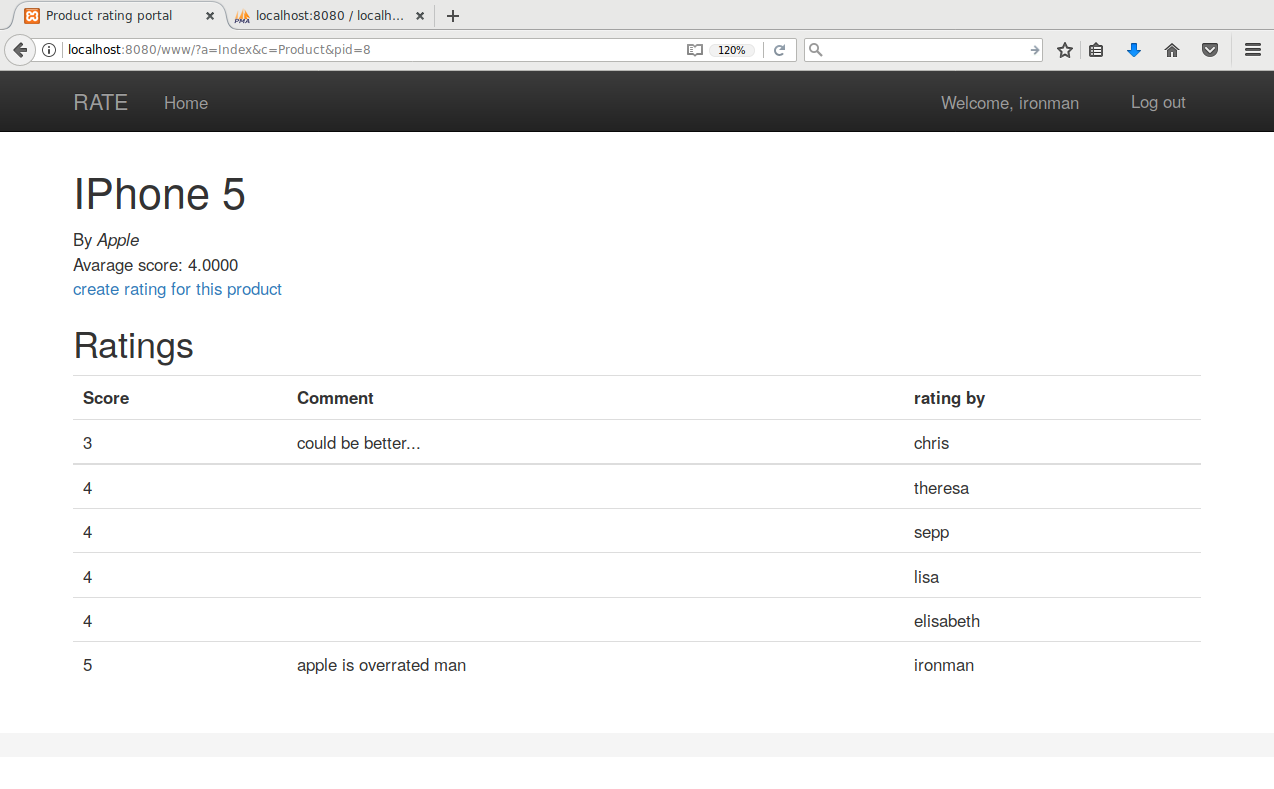
\includegraphics[width=1.0\textwidth]{7.png}

Übersicht über die eigenen Produkte und Bewertungen.

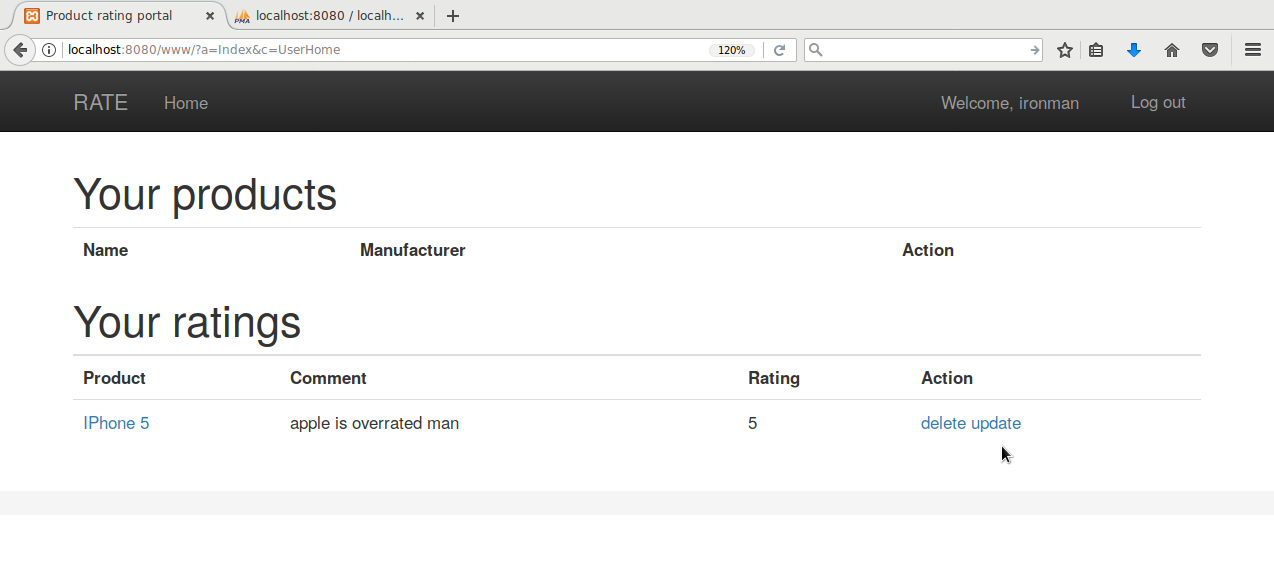
\includegraphics[width=1.0\textwidth]{8.png}

Änderung einer Bewertung.

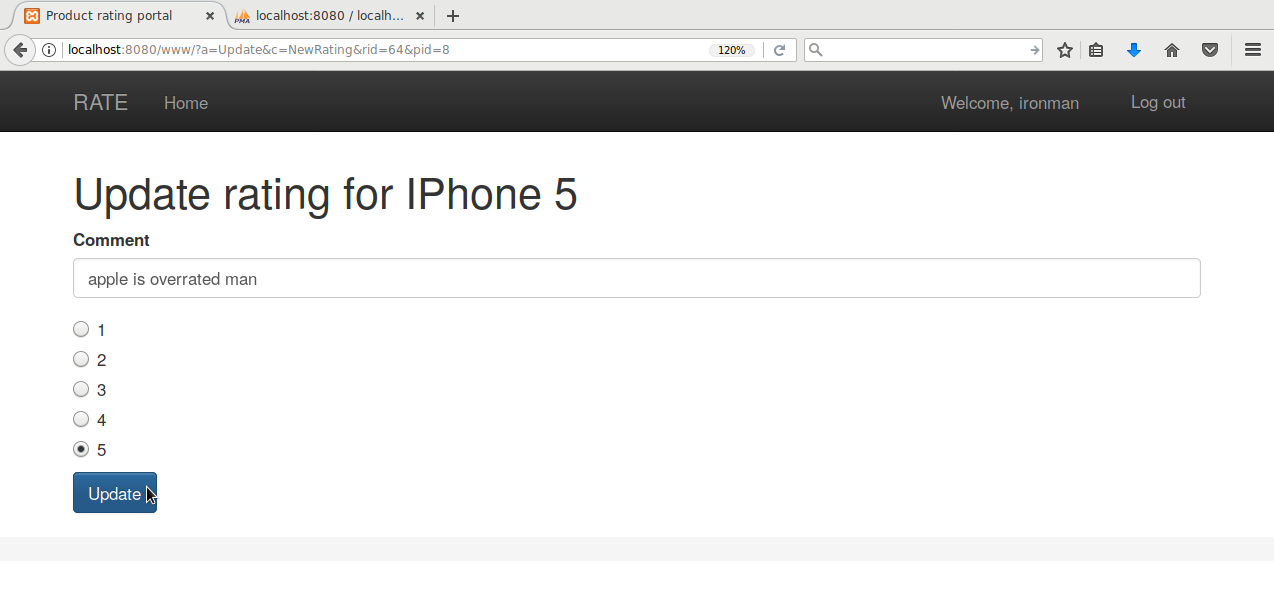
\includegraphics[width=1.0\textwidth]{9.png}

Datailansicht nach Änderung.

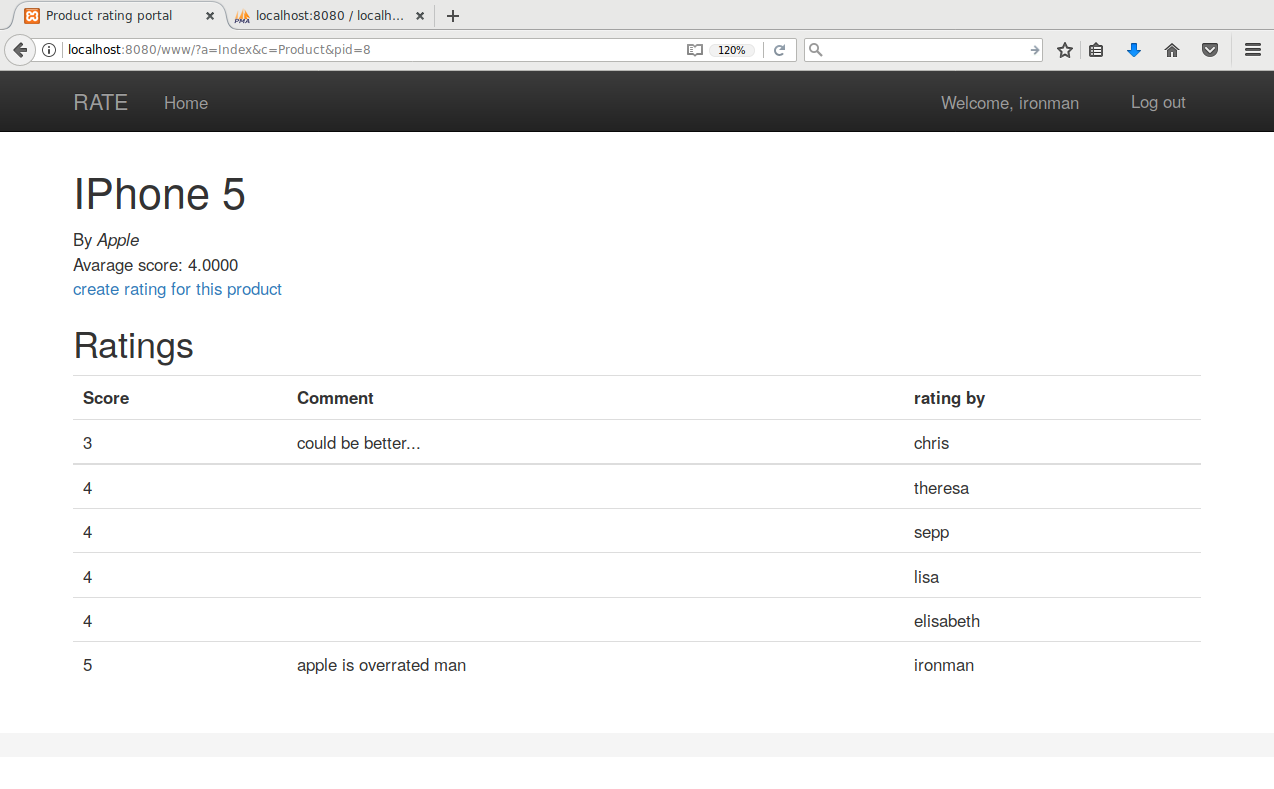
\includegraphics[width=1.0\textwidth]{10.png}

Detailansicht im ausgeloggtem Zustand.

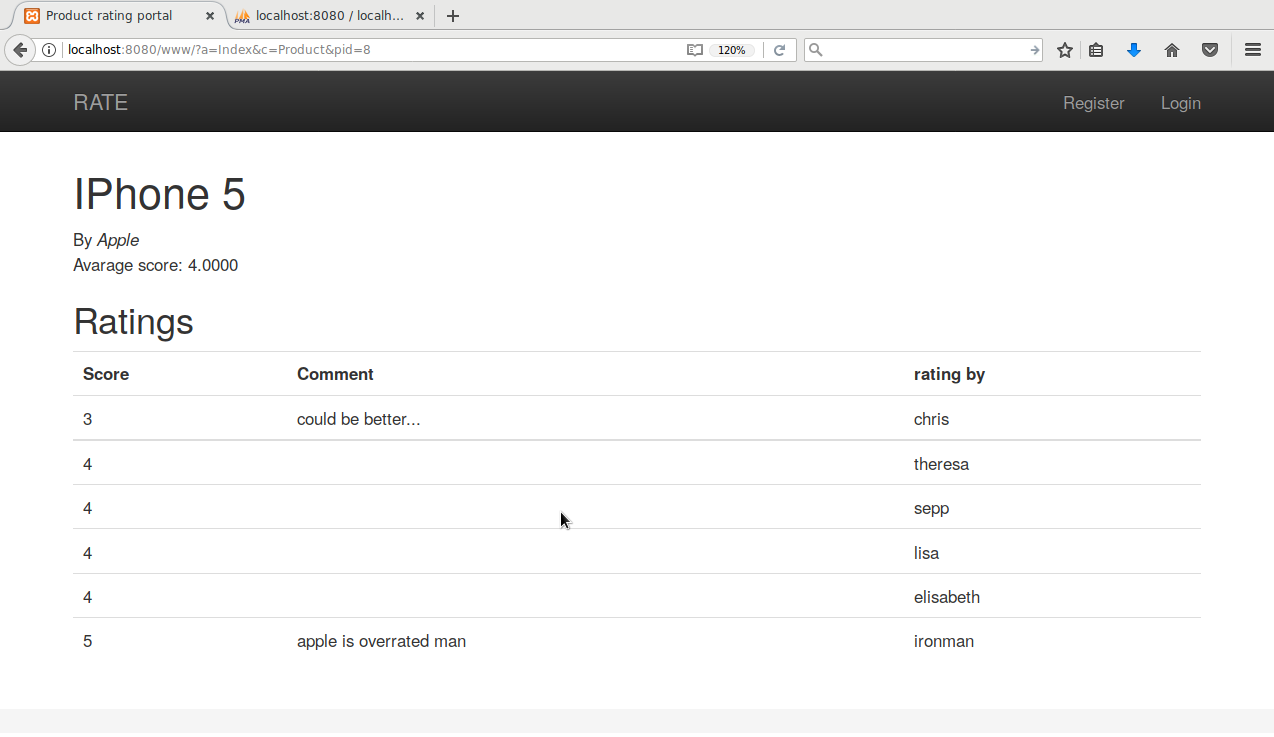
\includegraphics[width=1.0\textwidth]{11.png}



\end{document}